%________________________________________________________________________________________________
\documentclass{beamer}
%________________________________________________________________________________________________
\usepackage[french]{babel} 
\usepackage[utf8]{inputenc} 
\usepackage[T1]{fontenc} 
\usepackage{graphicx}
\usepackage[utf8]{inputenc}
%\usepackage{sectsty}
\usepackage{fancyhdr}
\usepackage{geometry}
\usepackage{tabularx,tabulary}
%________________________________________________________________________________________________
\title{3I013 Réunion du 8 Mars 2019}
\author{Daoud KADOCH\\Fabien MANSON\\Maël FRANCESCHETTI\\Nicolas CASTANET\\}
%________________________________________________________________________________________________
%ce theme est le plus clean de Beamer le truc a ne pas utiliser c'est 'Warsaw'
\usetheme{default}
%suppression de la barre de navigation inutile
\setbeamertemplate{navigation symbols}{}
\setbeamertemplate{frametitle}[default][center]

%\logo{
\includegraphics[height=0.5cm]{logo_sorbonne.png}}

%________________________________________________________________________________________________
\addtobeamertemplate{footline}{
	\begin{flushright}
	\vbox{\insertframenumber/\inserttotalframenumber}
	\end{flushright}}

%________________________________________________________________________________________________
\begin{document}
	%____________________________________________________________________________________________
	\begin{frame}
		\begin{center}
		\maketitle
		
\includegraphics[height=0.7cm]{logo_sorbonne.png}
		\end{center}
	\end{frame}
	%____________________________________________________________________________________________
	\begin{frame}
		\begin{center}
		\frametitle{Sommaire}
		\tableofcontents{}
		\end{center}
	\end{frame}
	%____________________________________________________________________________________________
	\begin{frame}
	\section{L'Objectif du Projet}
		\begin{center}
		\frametitle{L'Objectif du Projet}
		%\subsection{Objectif}
        %\framesubtitle{L'expression des besoins}
		   Faire effectuer une ronde à un drone Bebop 2 en suivant un itinéraire prédéfini, tout en visualisant le retour vidéo en temps réel sur un iPod à travers un masque FPV.
		\end{center}
	\end{frame}
	%____________________________________________________________________________________________
	\begin{frame}
	\section{Use Case}
		\begin{center}
		\frametitle{Use case}
		%\subsection{Use Case}
        %\framesubtitle{L'expression des besoins}
        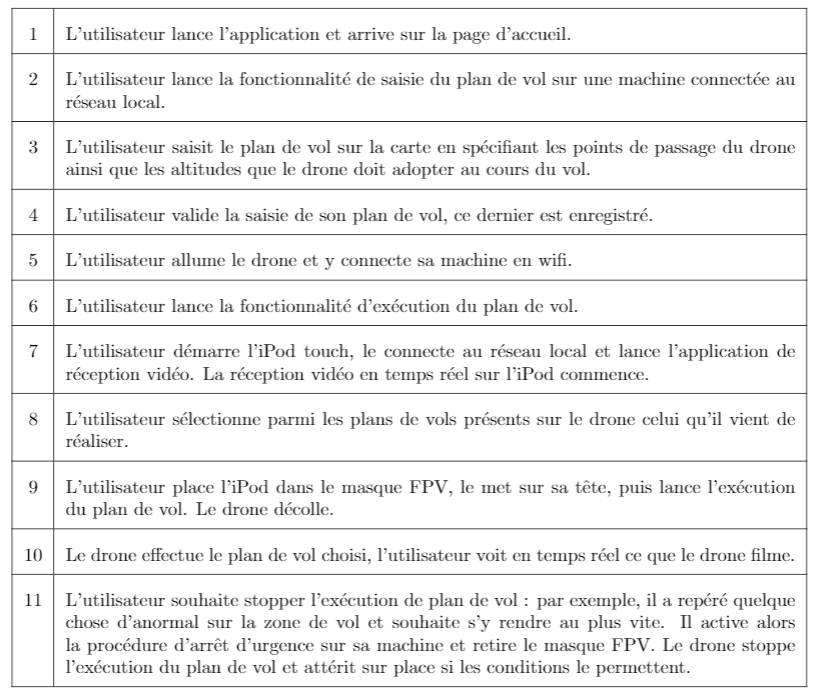
\includegraphics[scale=0.52]{Use_Case.PNG}
       \end{center}
	\end{frame}
	%____________________________________________________________________________________________
	\begin{frame}
	\section{Les Besoins Fonctionnels}
		\begin{center}
		\frametitle{Les Besoins Fonctionnels}
		%VERSION FM		
        %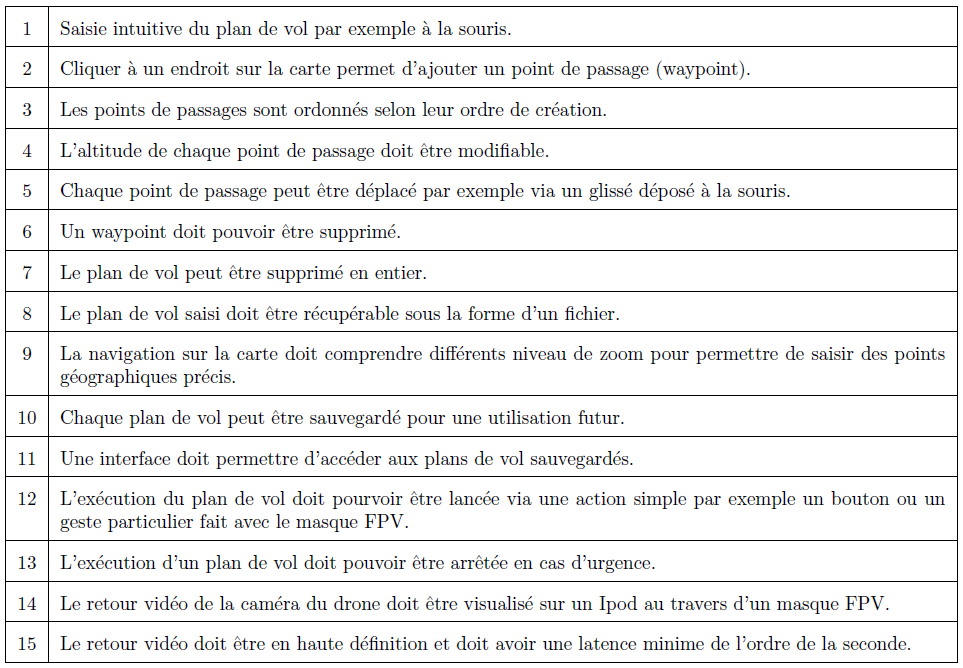
\includegraphics[scale=0.42]{tableau_des_fonctionnalites.png}
		%VERSION DK		
		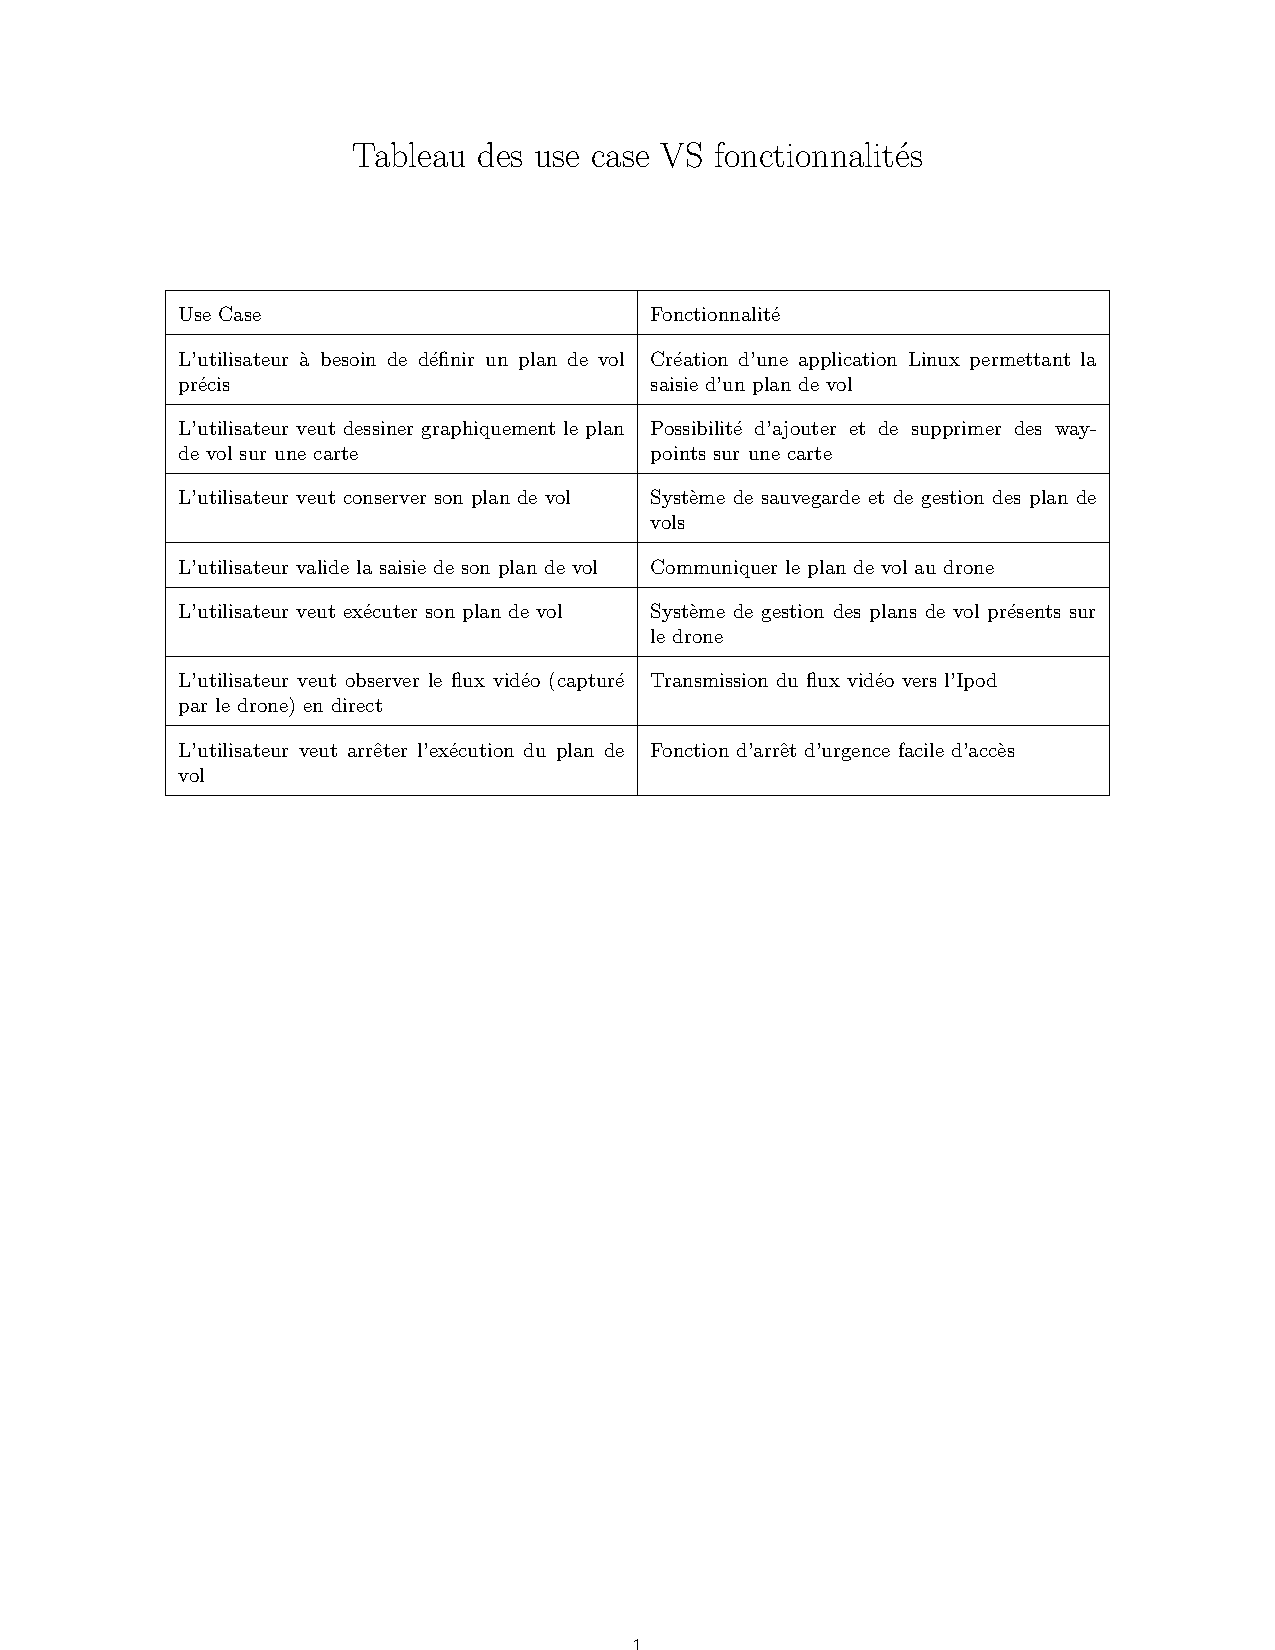
\includegraphics[scale=0.47]{use_charges2.png}
				\end{center}
	\end{frame}

	%____________________________________________________________________________________________
	\begin{frame}
	\section{Les Solutions Étudiées}
		\begin{center}
		\frametitle{Les Solutions Étudiées}
		%\subsection{Les Solutions étudiées}
        %\framesubtitle{Les solutions}
        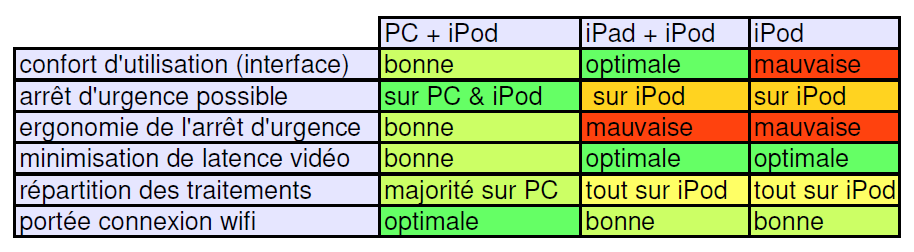
\includegraphics[scale=0.45]{comparatif_v2.PNG}
		\end{center}
	\end{frame}
	%____________________________________________________________________________________________
	\begin{frame}
	\section{Les Contraintes}
		\begin{center}
		\frametitle{Les Contraintes}
		%\subsection{Contraintes}
        %\framesubtitle{Les solutions}
           	\begin{itemize}
                \item Matériel : Bebop2, PC Linux, iPod
                \item Un réseau local connecté au PC et à l'iPod, et bénéficiant d'un accès internet (API carte)
                \item Saisie du plan de vol ergonomique, simple, intuitive
                \item Arrêt d'urgence depuis le PC
            \end{itemize}
		\end{center}
	\end{frame}
	%____________________________________________________________________________________________		
	\begin{frame}
	\section{La Solution Retenue}
		\begin{center}
		\frametitle{La Solution Retenue}
		%\subsection{Solution retenue}
        %\framesubtitle{Les solutions}
            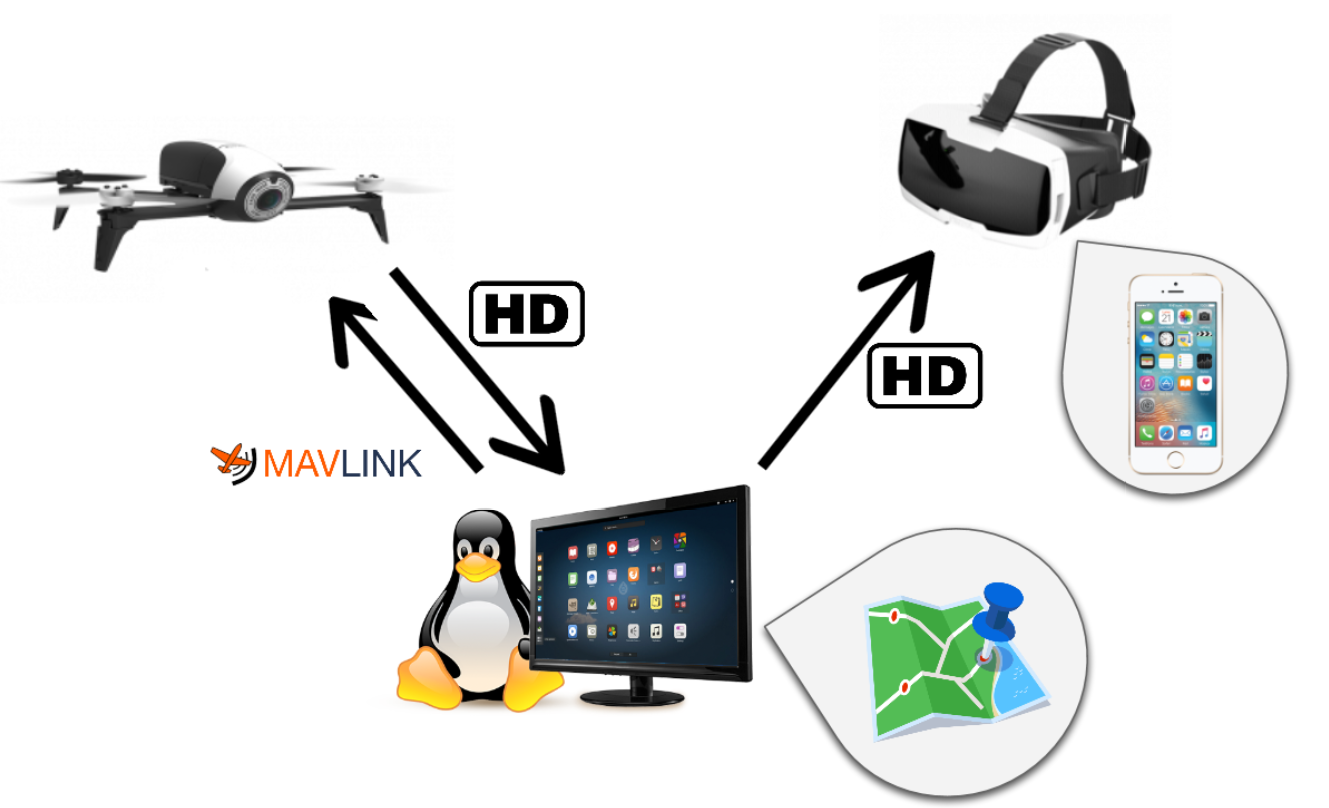
\includegraphics[scale=0.45]{schemaPC.png}
		\end{center}
	\end{frame}
	%____________________________________________________________________________________________
	
\end{document}
%________________________________________________________________________________________________